\section{Designing GCom middleware}

\paragraph{}{
	The GCom application is basically made up of three layers as
 we can see on figure \ref{fig:architecture}.
 Each layer has different responsibilities. The layers allow 
 making abstraction and shared out responsibilities.
}

\begin{figure}[!ht]
	\begin{center}
	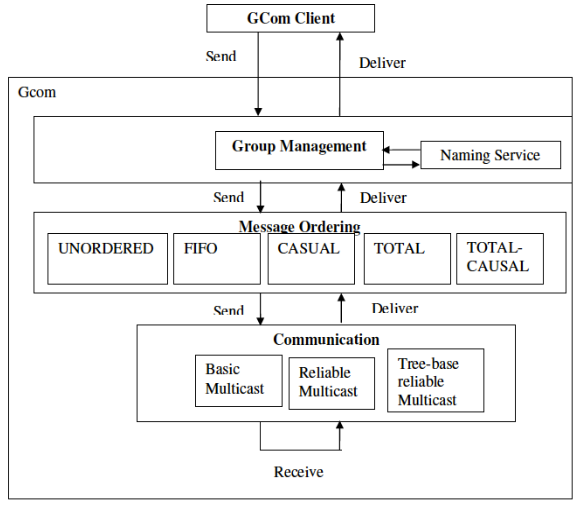
\includegraphics[width=0.7\textwidth]{figures/gcom_architecture.png}
	\end{center}
	\caption{Global architecture of GCom middleware}
	\label{fig:architecture}
\end{figure}

\paragraph{Group management}{
	The top layer is the part tasks with the group management.
 The group management elects a new leader, adds and removes
 members within the group, handles errors and notify processes
 about group changes.
}

\paragraph{Message ordering}{
	The message ordering layer determines in which order
 messages are delivered to the next layer according different
 strategies. For instance, we can order messages according to the
 "First In, First out" policy, use a causal order or a mix
 between two existing ordering like Total-Casual.
}

\paragraph{Communication}{
	The communication service is the lowest level. It deals
 with the Java RMI objects. It allows different type of
 communication like multicasting and, maybe, a tree based
 communication. \newline
 Moreover, the debug interface will be mainly implemented here.
}

\paragraph{Debugging}{
	Additionally, the communication module offers an interface
 to set up how to simulate network latency and failures.
}

\paragraph{Naming service}{
	To get into the group, or at least ask to group to join,
 we need a service to solve how to find a group on the network.
 It is basically the entry point of the system.
}
